\section{Start rescue system}If you want to start a client for repairing or diagnostic purpose, you can boot the rescue system over the network. After the network boot the client starts a console that allows you to do your work. To start the rescue system click on \textit{"Rescue system"} after the client name.\\
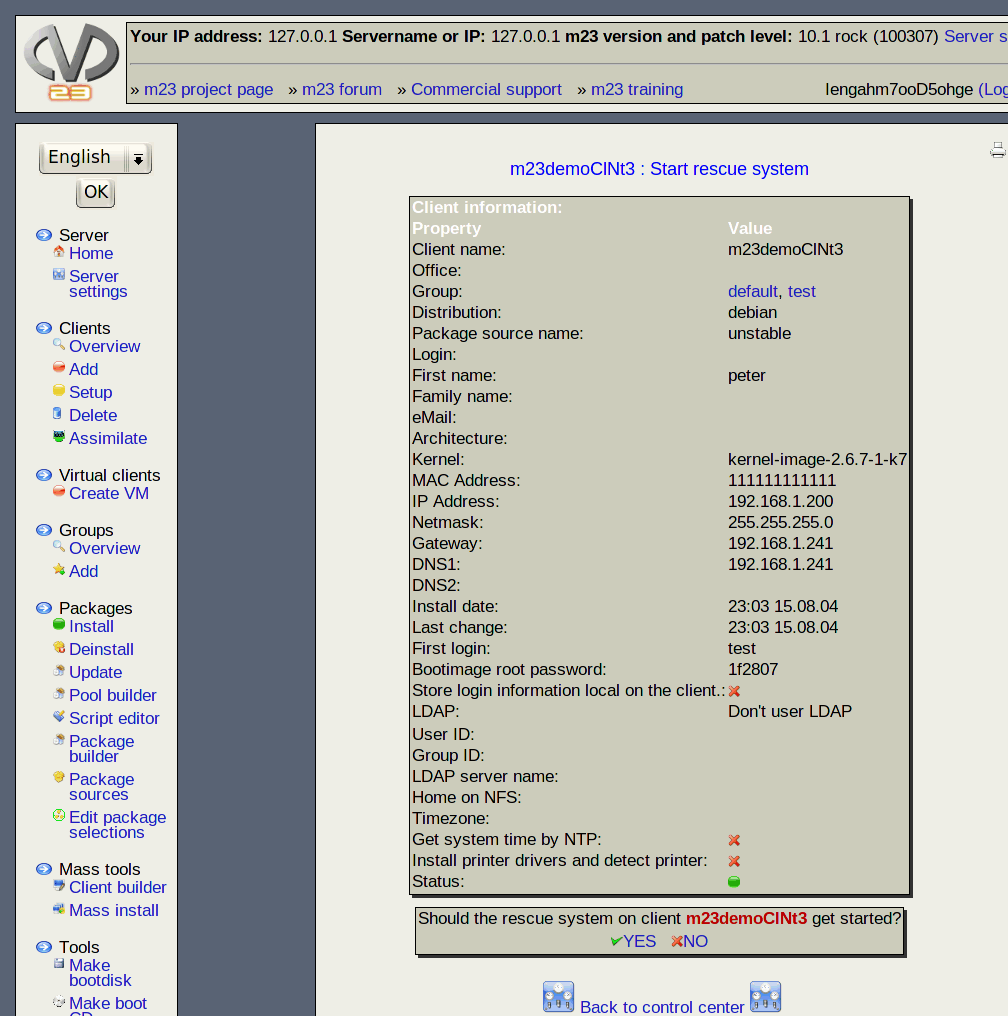
\includegraphics[scale=0.4]{/mdk/doc/manual/screenshots/en/rescue_client.png} \\
\subsection{Hint}:\\
The rescue system will be started every time you boot the client until you delete the "m23Rescue" job from the job list. You can find the list  on the page \textit{"Clients overview"} if you click on the number in the "Jobs" line.\\
